\documentclass[10pt,twocolumn]{article}
\usepackage{nffs}

\author{Roie R. Black}
\date{\today}
\title{Designing an Indoor Model using OpenSCAD}
\titlepic{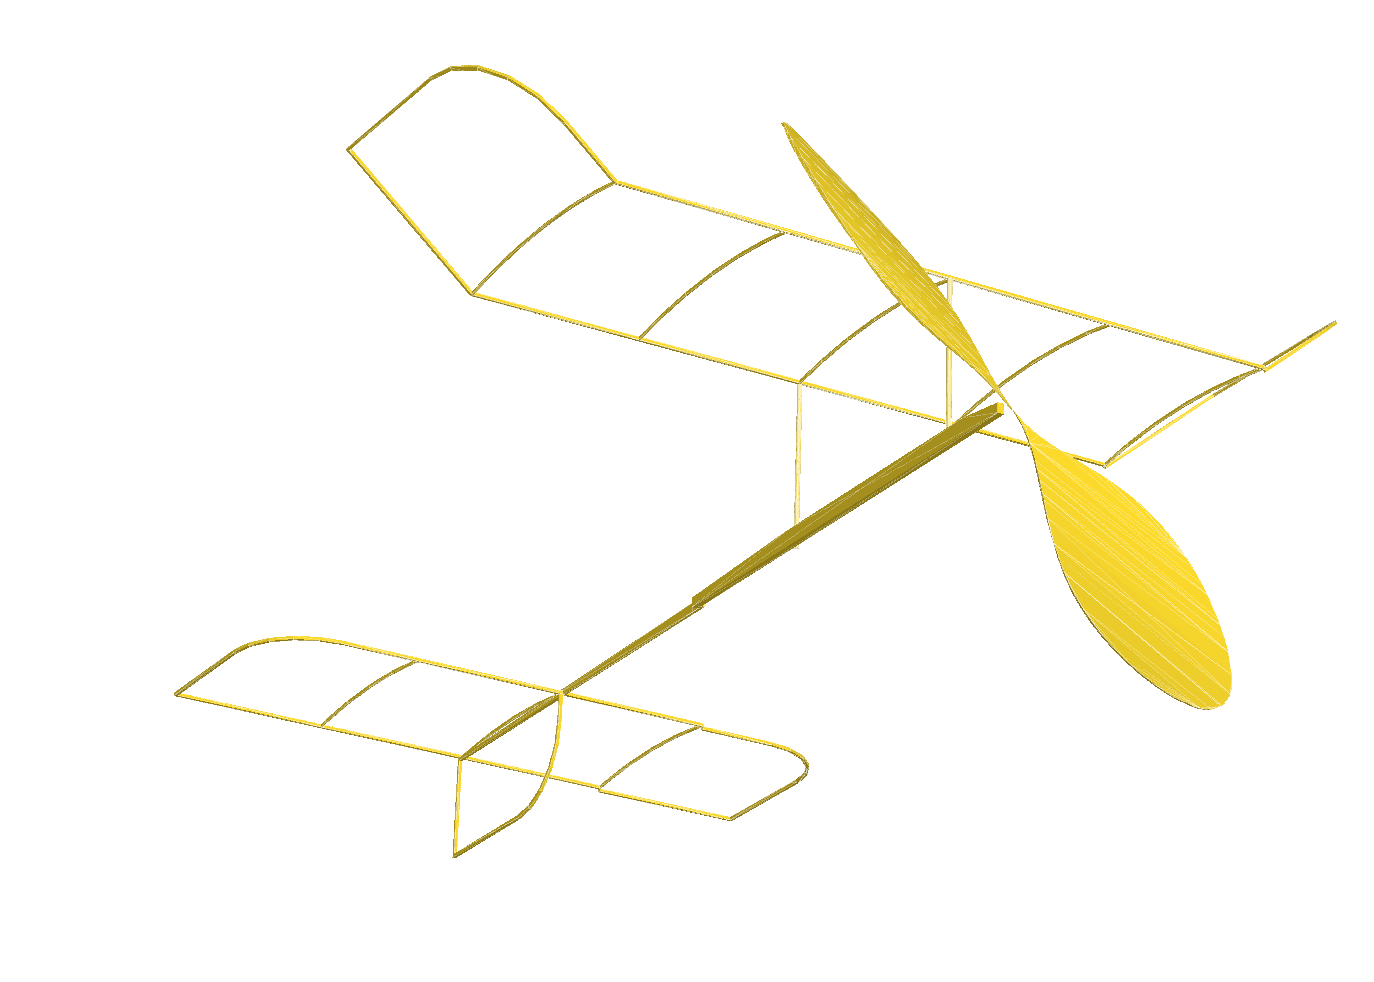
\includegraphics[width=0.66\textwidth]{./assets/images/math-magik-lpp.png}}


\begin{document}
\maketitle

Designing a new model airplane usually involves generating a plan of some sort,
then constructing a prototype model from that plan. Of course you can use a
pencil and paper to generate your plans, but if you think you might want to
publish the plan, you will need to use some form of {\it Computer Aided Design}
tool to produce your final plan. Unfortunately many popular CAD tools are
complex, and often too expensive for the average modeler.

Having recently retired from teaching Computer Science, and finally getting back into
model building, I decided to design a new indoor model for the {\it Limited
Pennyplane} class. As part of the design process, I wanted to see that airplane
in 3D even before I built the first prototype. I decided to use a different
form of CAD tool: OpenSCAD \cite{openscad}, a tool designed for computer
programmers!

While that description may discourage some folks from reading further, rest
assured that this particular tool is simple enough that non-programmers can
certainly master it. In fact, some teachers have successfully managed to get
elementary school kids to use OpenSCAD to design simple 3D models.

OpenSCAD is an open-source (meaning free) 3D modeling program, available on all
major platforms. It is commonly used by folks designing parts to be printed on
3D printers. What makes OpenScad different is how you generate the design.
Instead of using your mouse to drag things around on the screen, you describe
your model in a simple programming language. Formally, OpenSCAD uses something
called {\it Constructive Solid Geometry} to construct your model, then gives
you a visual interface you can use to examine your 3D model in detail.

I will only show example code from the project so you can get a feel for the
design process. You are encouraged to explore the project website for much
better documentation and complete source code. \cite{blackr}.


\section{OpenSCAD}

Installing OpenSCAD is oretty simple using instructions found on the projects
website. Once it is installed, open it up and take a look at the basic
interface:

\importimage{opening-screen}{OpenSCAd interface}

There are three areas we will be using in this view:

\begin{itemize}
\item{Editor - the left panel where you type in your code.}
\item{Preview - the top right panel will be where your model is displayed.}
\item{Messages - the bottom right panel is where error messages will be shown
when processing your code.}
\end{itemize}

I will not try to show everything you need to know about the language {\it
OpenSCAD} uses for describing a model. Instead, I will show fragments of code
to give you a feel for what you need to write to design your model. The project
website~\cite{blackr} has more details, as does the {\it OpenSCAD} {\it User
Manual}~\cite{userman}.

A Handy ``cheat-sheet'' is available here:~\cite{osccheat}.

\subsection{Organizing Your Code}

\osc\ lets you write your code in one file or in multiple files. I like to
split up a design into multiple files in order to keep them short and focused
on one just part of the design. If you split things up you will need to use either
an {\it include} or a {\it use} line specifying the file you want to access with
the code in the present file. If you choose {\it include}, all that code in the
second file will be processed as though it had been typed in the current file.
On the other hand, using the {\it use} line only makes the names from the
second file available in this one. The code in the second file will only be
processed when those names are encountered in the current file.

A typical setup is to create a single file with variables you want every piece
of code to be able to use. You {\it include} that file like so:

\begin{lstlisting}
include <m th-magik-data.scad>
\end{lstlisting}

Another example might be in a file defining the wing for this design. That file
needs to use ribs, which I define in another file. In my wing file I would
add this line

\begin{lstlisting}
use <rib.scad>
\end{lstlisting}

You will see a lot of this notation in the full project code files on the
project website.

\subsection{The Designng Process}

Building a 3D model is a trial and error process. You type in or modify your
code, then click on a command to process that code. You look at the preview
window to see your model, and search the message area for hints about what went
wrong.  Non-programmers will find this a bit frustrating, but this takes
practice to master, so do not get discouraged. My advice is to always take
small steps.  That limits the number of problems you face in getting things to
work.

The best way to learn anything new is to experiment. Beginning programmers are
always searching the Internet for solutions they can copy into their problems,
but the only thing you actually learn when copying and pasting stuff is how to
copy and paste. You will learn far more by typing in code yourself - at least
until you get more proficient at this. Reading the code gives you a chance to
really think about what is going on. There is nothing wrong with looking at
code written by others. Many times studying that code will teach you how to
better write your own code. I will show you enough code in this design to give
you a feel for how you do things using \osc. The actual code I generated for
this design is on the project Github account~\cite{blackr}.

I highly recommend building small files that generate one part of your overall
design. Test that component until you are sure it looks like what you want.
Then use that part in building other components. I like to work from small
parts up to bigger assemblies, and that is how we will work through this
design. Don't be afraid to fire up \osc\ and try things are you read this
article. Of course, you should look at the project website to see all the code
in greater detail.


\section*{\mbox{Constructive Solid Geometry}}

OpenSCAD builds 3D models using a small set of primitive shapes, and a set of
movement and combining operations to create more complex models.

\subsection*{Primitive Shapes}

Openscad supports both 2D and 3D shapes. We will be using some simple 2D
shapes, like circles and rectangles, and more complex 2D shapes like a polygon.
The 3D shapes we will use include spheres, cylinders, and cubes. All of these
shapes can be scaled and moved around using simple movement operations.

\subsection*{3D Primitives}
For our first look at how you do things in OpenSCAD, here is a piece of code
that will show the three basic 3D shapes:

\includecode{demo/demo1.scad}

Figure \ref{fig:demo1.png} shows the result.

\importimage{demo1.png}{Demo 1}

Each primitive shape is created at the origin. Cubes are created in the region
where all three coordinates are positive. Spheres are created with the center
of the sphere at the origin. The cylinder is centered along the {\bf Z} axis.
If you look closely, you will see a small representation of the coordinate
directions at the lower left of this image.

We used a {\it translate} operation to move shapes aside so they do not
overlap. The numbers inside square brackets control the distance we want to
{\it translate} the following shape in the {\bf [x,y,z]} directions. This
bracketed group of numbers is is called a {\it vector} which we will use a lot
in our work.

Notice how I indent code to show how things happen. In this example, we {\it
translate} the following {\it cube} shape. The semicolon ends this command.
Failing to put semicolons where they are needed is a common mistake when
writing \osc\ code.

These shapes do not look quite right. The problem is that \osc\  generates
approximations to the rounded shapes, using a set of small polygons to build up
the model. If we make these polygons smaller, things look better. All we need
to do to fix this is change the code so it looks like this:

\includecode{demo/demo2.scad}

Figure \ref{fig:demo2.png} shows a much better result. The special variable
{\it \$fn} controls the resolution of rounded objects. Bigger numbers make
things look smoother but cost of longer times to generate images on the screen.


\importimage{demo2.png}{Demo 2}

Some shapes are smart and can form different versions of themselves:

\includecode{demo/demo3.scad}

Figure \ref{fig:demo3.png} shows a warped cube and cylinder. Spheres are not so
smart, they stay spheres unless we warp them with external commands.

\importimage{demo3.png}{Demo 3}


\subsection*{2D primatives}

We will use a few 2D shapes in this design, including the circle and square,
which act much like their 3D counterparts. A more interesting 2D shape we will
use is the {\it polygon}.

\includecode{demo/polygon-demo1.scad}

Here, we create two {\it variables} and set them equal to a list of vectors. 2D
vectors have only 2 numbers, for the {\bf X} and {\bf Y} coordinate values. The
first list defines a set of six points: three for the outer triangle, and three
more for the inner triangle. The second list identifies {\it paths} meaning a
continuous line that makes up a closed circuit, one for the outer triangle, and
one for the inner triangle. The numbers refer to the position of vectors in the
first list (programmers count starting at zero!) That final {\bf 10} parameter
is not important here, it helps the operation work properly.

I know this is a bit confusing, but we will not need much of this kind of code
in our design work. Remember to try things and see what happens.

\importimage{polygon-demo1.png}{Polygon Demo 1}

Figure \ref{fig:polygon-demo1.png} shows a  2D shape with no thickness, although
\osc\ gives it enough of a thickness to show up on the screen.

We can use this 2D shape to create a 3D object by {\it extruding it} in the
{\bf Z} direction:

\includecode{demo/polygon-demo2.scad}

Figure \ref{fig:polygon-demo2.png} definitely shows an interesting shape. We
will use {\it extrusion} to make some parts that would be difficult to construct
with just the basic primitive shapes.

\importimage{polygon-demo2.png}{Polygon Demo 2}

Obviously, we can form some interesting things with \osc. But things get
even more interesting when we start combining multiple shapes to form more
complex objects.

\subsection*{Movement Operations}

We saw the {\it translate} operation earlier. We can also {\it rotate} a shape.
In this command we provide a vector of angles (in degrees) that we want to use
to rotate the shape. Each number in the vector will be used to rotate the shape
around the coordinate axis associated with that number. For instance {\bf
rotate([90,0,0])} will rotate the shape around the {\bf X} axis ninety degrees.
This operation uses the {\it right-hand} rule. If you want to rotate around the
{bf X} axis, take your right hand and point the thumb in the direction of
increasing {\bf X} in your coordinate system. Your fingers ``curl'' around that
axis in a positive direction.

Combining translations and rotations is done by writing both commands like
this:

\begin{lstlisting}
  translate)[10,15,0])
    rotate[90,0,0])
      cube(1,1,5);
\end{lstlisting}

It helps to read this bottom up. We are creating a {\it cube} at the origin. We
rotate it so it is aligned the way we want, then we translate that result to
the position we have chosen. The semicolon at the end of this list ends the
command. Notice that I indent so show what I want my code to do.

Be warned that you can swap the {\it translate} and {\it rotate} commands, but
you might not get the result you expect. Rotations are applied to the shape as
it is positioned when the command is processed. If you rotate after
translating, The shape will swing a long way!

\subsection{Combining Operations}

We form more complex objects by moving things around and combining them to form
new objects. An example found in the {\it Wikipedia} article on CSG~\cite{csgwiki}
demonstrates these operations.

Suppose you wanted to build something that looks like Figure \ref{fig:csg-demo.png}.

\importimage{csg-demo.png}{CSG Example Shape}

We can form this shape using three cylinders, a sphere, and a cube. We use all
three basic combining operations to construct the final shape.

Here is the OpenSCAD code used to generate this shape:

\includecode{demo/csg-demo.scad}

There is a point to be made here. We can move two objects together so they
touch, like a rib to a spar, but we do not really need to join them together in
this design work. Visually, things will look right, but the two objects remain
separate. Joining them together to make a combined part would be important if we
were going to 3D print the object. Since we do not have he technology to print
with balsa (yet), I will not worry about combining the components of our design
to create a single airplane object.

\subsubsection*{Modules}

\osc\ lets you package a number of operations in a {\it module} that you can
activate later, one or more times. In fact those primitive shapes were all
predefined {\it modules}. The module can have parameters, which makes this a
powerful way to manage shapes that are similar, but differ depending on the
parameters you specify.  We saw that when we showed ``warped'' shapes earlier.
We will create a basic rib module for this model, and use parameters to control
the exact rib we want.

All modules have a unique name in your code.  The name you choose should help
you remember what the module is all about. In this example, we are interested
in the final {\bf part} shape, which is constructed using the difference
operation. This final module uses two supporting modules to build the part. You
can write your code almost any way you like, but it is common to use
spaces,indentations, and newlines to organize your code to make reading it
easier.  Also, we surround a sequence of individual operations inside of curly
braces when needed. I always indent any code inside of these braces.

When you add parameters to a module, you define names for each one between the
parentheses. Commas separate parameters if you have more than one. You can
optionally provide a default value for each parameter by adding an equal sign
followed by the default value you want. When you activate the module, you must
provide actual values you want the module to use. You can just provide a
sequence of numbers in the right order with commas separating them, or you can
add the parameter name from the definition, an equal sign, then the new value
you want. In this case, the order is not important, and you can leave off any
parameters where you are happy with the default value.  The rules for all of
this are detailed in the \osc\ {\it User Manual} \cite{userman}, so I will
not go further in this discussion here.

\subsubsection*{Building the Example Shape}

To build this part, we first set up three cylinders, aligned along each
coordinate axis. The {bf center} parameter, sets each cylinder up with the
origin of the coordinate system at the exact center of the cylinder. Remember, The {\bf
\$fn=32} parameter is really only needed to make the cylinders actually look
round.

Notice that all three of these cylinders occupy the same space. In the real
world, we could not do that, but in our 3d modeling world this is common. We form
the {\bf union} of these three overlapping cylinders to form one merged shape.

The outer shell of our part is made up of the {\bf intersection} of a sphere
and a cube. We size the cube shape so it trims off six sides of the sphere
where holes will end up.  Finally, we use the {\bf difference} operator to
carve out the inside of the part, using our three-cylinder shape.

Successfully building 3D models involves visualizing what you want, then
arranging simple shapes as needed and performing these three basic combining
operations to generate the gadget you want! It takes practice! The more you
experiment the better you will get!

I encourage you to fire up \osc\ and type in this code. You will be better
able to see how things work by doing this!

\section{Design Constraints}

The {\it Limited Pennyplane} class rules define a few constraints on dimensions
for our model. Specifically we must honor these limits:

\begin{itemize}
\item{{\bf max\_wing\_span} -  18''}
\item{{\bf max\_wing\_chord} -  5''}
\item{{\bf max\_stab\_span} - 12''}
\item{{\bf max\_spab\_chord} - 4''}
\item{{\bf max\_length} - Max Prop to Tail length = 20''}
\item{{\bf max\_prop\_diameter} - 12''}
\end{itemize}

What this means is that the model must fit in a box that measures {\bf
max\_wing\_span} wide by {\bf max\_length} long. There is no limit on how
tall this box can be.

Furthermore, the wing must fit in a smaller box measuring {\bf max\_wing\_span}
by {\bf max\_wing\_chord}. The stabilizer must fit in a similar box measuring
{\bf max\_stab\_span} by {\bf max\_stab\_chord}. There are no constraints on where
these boxes fit inside the outer box. The propeller is only limited by
diameter, blade shape it up to the designer. However, the {\bf max\_length}
constraint is measured from the forward-most point, usually on the propeller,
to the aft-most point on the model. We could build a pusher, but I have not
considered that idea.

\importtikzfigure{lpp-design-constraints}{LPP Design Constraints}

Note: The labels in this diagram are abbreviations for the names shown above.
In my code I will use full names to improve readability of the code.

input{wing}
\section*{Stabilizer and Fin}

The code we created to build the wing provides everything needed to build the
stabilizer and fin.

\subsection*{stabilizer}

The stab is identical to the wing, except in dimension ans
number of ribs. The modules used for the wing give us everything needed to
build the stabilizer.

Figure \ref{fig:stab.png} shows the result.

\importimage{stab.png}{Stabilizer}

\subsection*{Vertical Fin}

The fin is a slightly different version of the tips. The only addition here is
a square spar at the base of the fin. As we will see, we will mount the fin at
an offset, and not glue it directly to the tail boom.

Figure \ref{fig:rudder.png} shows the fin.

\importimage{rudder.png}{Vertical Fin}


\subsection{Motor Stick}

With the flying surfaces set up, we can now turn to the fuselage parts. The
most important of these is the motor stick, which supports everything else in
the model. The motor stick must also bear the forces imposed by the wound up
rubber motor that will power this craft.

We can set up the motor stick several ways, but I will use a {\it polygon} to
define the basic shape, then use {\it linear\_extrude} to generate the actual
object.

Here is the basic layout we will use:

\importtikzfigure{motor-stick}{Basic Motor Stick}

This design provides support for the front bearing and the rear hook. The
module only needs one parameter: the thickness of the stock you will be using
for this part.

\begin{lstlisting}
module motor_stick(thickness=1/8) {
  ...
}
\end{lstlisting}

The final shape is centered along the {\bf X axis} with the bottom of the stick
lying on that axis to make final assembly of the model easier.

\importimage{motor-stick.png}{motor-stick.png}

I added one new feature to this module, which will not show up in the printed
article. You can ask \osc\ to color shapes using the {\it color} command. For
this motor stick, I just added this code to the module:

\begin{lstlisting}

module motor_stick*thickness=1/8) {
  color(WOOD_Balsa)
    rotate[(90,0,0)])
      translate([0,0,thickness/2])
  ...
}
\end{lstlisting}

I also added a single line at the top of the file:

\begin{lstlisting}
include <colors.scad>
\end{lstlisting}

The {\bf colors.scad} file is one I found online. I added my own color for balsa!


\subsection{Tail Boom}

After building the motor stick, the tail boom is something of a letdown. All we
need here is a basic stick, but tapered from the front to the rear.

\begin{lstlisting}
module tail_boom(
	thickness = 1/16,
	front_height = 3/16,
	rear_height = 1/16
	) {
  ...
}
\end{lstlisting}

We will see this part when we assemble the airplane

\subsection{Propeller}

Now for an interesting component - the propeller. This is not just a flat part,
it has an interesting shape, and figuring out how to model this thing took some
time. In the end, I remembered how most of us build indoor propellers. We take a
thin sheet of balsa, cut out the blade profile we want, then soak that blade
for a while. Next, we tape it to the side of a round can at an angle and bake
it. When it dries, it has a curvature that will work fairly well.

It struck me that I could generate the same shape by creating a polygon that
represents the blade outline, then extrude that to form a very thick blade
(bigger that the can!) I then build a hollow cylinder with a thickness that
matches our desired blade thickness and slide the extruded blade into that cylinder.
The {\it intersection} of these two shapes will leave us with a curved blade.
Neat!

The shape of the blade seems to be a matter of taste. Many builders design
blades that will provide for a flair so that the prop will have a higher pitch
when the plane is launched with full torque from the motor. Moving the prop
spar toward the trailing edge of the blade provides this flair.

I decided to generate a simple blade layout, with parameters that can be
adjusted to give the flair you want. Figure \ref{fig:prop-blade} shows the
general layout.

\importskinnytikzfigure{prop-blade}{Prop Blade Layout}

The prop spar is a tapered cylinder, something easy to generate with the {\it
cylinder} shape. Parameters are provided so the size of the spar can be
adjusted.
i
Figure \ref{fig:prop-blade.png} shows the final blade produced. Since the code is
again a bot complicated, I will refer you t the project website.

\importimage{prop-blade.png}{Prop Blade}



\subsection{Final Assembly}

Now that we have all of the major components defined, it is time to put things
together and see the completed model.

\subsubsection{Mounting Components}

The wing will be mounted on top of two hard balsa posts using paper tubes.
These wing posts are glued to the motor stock on the bottom and rounded at the
top to slide into paper tubes that will be glued to the wing structure.

A similar arrangement is used to attach the stabilizer on top of the tail boom.

The rudder is glued to the bottom on the tail boom, but is offset to provide for
a turn during flight. A small stick of balsa will be glued to the rear of the
tail boom and the fin to provide needed support. Should this need adjusting,
the rear attachment can be unglued and repositioned.

\subsubsection{Paper Tubes}

Paper tubes are formed on a mandrel using a strip of tissue soaked in thin
glue and twisted around that mandrel. The resulting tube, after pulling off of
the mandrel, will be stiff enough to provide the support needed. The posts must
be carefully sanded to ensure a tight fit.

The code that creates a paper tube, it is just a very skinny hollow cylinder.

Figure \ref{fig:wing-mount-tube.png} shows an image showing how the tubes are attached
to both the wing and stabilizer:

\importimage{wing-mount-tube.png}{Wing Mount Tube}

\subsubsection{Mounting Posts}

The posts used to attach the wing and stabilizer are simple sticks of hard balsa with
rounded tops that are sized for a tight fit in the paper tubes.

Since we need several mounting posts, the code that generates the post is
placed in another module:

To attach the wing, we need to attach two posts to the motor stick:


\subsubsection{Mounting Tail Group}

Both the stabilizer and fin mount on the tail boom.

\subsubsection{Stabilizer}

The stabilizer is mounted on top of the tail boom, using small posts and paper
tubes to allow for minor adjustments when flying.

\subsubsection{Vertical Fin}

The rudder is simple attached to the bottom of the tail boom, Since that side
of the boom is canted by the trimming we performed earlier, we need to rotate
the rudder slightly during positioning.  However, we allow for  left rudder
attachment to provide a left turn flight path.

\subsubsection{Adding the Propeller}

We still need to set up the propeller. The wire parts need to be positioned,
then the propeller translated into place. I rotated the prop a bit so the final
image looks nicer. What you get us shown in the figure at the beginning of this
article.



\section*{Flight Box}

Since indoor model airplanes are so extremely light and fragile, it is
important that you give thought to how you are gong to transport the model.
Most builders do not show up at a flying site with just one model. Often, they
bring several for each event they want to fly. Many serious flyers build a nice
carrying case for their models. I decided to design one for Math-Magik!

When I was first getting into indoor competitions back in my college days, I
met Bud Tenny, who was the editor of a now-classic series of newsletters called
{\it Indoor News and Views}. These newsletters provided a wealth of information on
building indoor airplanes, and provided tips on how to fly them. Often there
were sketches of simple boxes made out of cardboard, or foam board that looked
like possibilities. However, I also have a copy of Ron Williams {\it Building and
Flying Indoor Model Airplanes} \cite{williams} , and ran into the ECIM
case, originally designed by the {\it East Coast Indoor Modelers} group. The design
presented here is a version of that case:

\importimage{flight-box.png}{Flight Box}


\subsection{Basic Construction}

As seen in figure \ref{fig:flight-box.png}, the box is made up of three
sections. One holds a number of wings (four are shown here). One holds the
stabilizers, and the middle section holds fuselages and propellers. The two end
sections are hinged to the center section so it opens as seen above. Closed,
this design measures 22"w x 9"h x 16"d. The outer sections are 6 inches deep
and the center section ins 4 inches deep.

The sides are constructed out of 1/8" plywood and all corners are braced with
1/2" pine strips. The hinges are piano hinges that run the full height of the
edges.

\subsection{OpenSCAD Design}

Designing this box with OpenSCAD turns out to be a nice way to figure out how
parts of the airplane will be transported and stored. The design of the
airplane structure presented so far allows both the wing and stabilizer to be
removed and stored separately. By attaching the wing posts to the motor stick and
using paper tubes for the attachments to flying surfaces on top of those posts,
the wings are not cluttered with structure and can be stacked neatly. The
stabilizers also stack nicely.

Laying the body on its side lets those be stacked as well.

That leaves the propellers! They can be stacked separately in the space above
the fuselage sections,.

When all of these items are placed in the box design, there is still room for
another model. My current thinking is to adds an A-6 model or two to this box's
payload!


\section*{Generating STL Files}

Many folks who use OpenSCAD generate {\it STL} files from their design. These
files are used as part of the 3D printing process. Although I wish we could 3D
print flyable model airplanes, that is not what we will do with the STL files
in this project.

STL stands for {\it Standard Tessellation Library} \citep{stlwiki}. Translated,
that means an STL file is a list of triangular objects that describe the
surface of a 3D object. These triangles cover the surface making a ``water
tight'' approximation to the real surface. Triangles are guaranteed to be flat
in the 3D space, and if they are tiny enough, they can be rendered to create a
3D display of the object, or sent to a 3D printer after suitable processing of all
the triangles so the printer knows where the surface is \(that is a topic for
another article!\)

My purpose in introducing these triangles is simple. I want to know how much my
model will weigh, and I want to know where the center of gravity will be when
the design is constructed. Figuring out these two details is impossible using
conventional building techniques: you build the model, weight it, and figure
out the center of gravity manually. Computer geeks never do anything manually
if they can get their computer to do the work.

I found a nice Python library that is all set up to figure out the volume of a
3D shape defined in an STL file, and return it's center of gravity location. It
is simple enough to add in the predicted wood density for the design and come
up with a weight estimate for each part. A little post-processing of all this
data will give us some estimate of the total designs weight. Unfortunately,
figuring out the weight of the glue is not so simple. For that we need to know
where each glue joint will be and the surface area of the glue joint. I am
working on that problem now, but am not ready to show any results yet.

Knowing where each part will be placed in the final design, and the CG data for
that part will let us predict the CG for the complete model as well!

Let's demonstrate this idea using a simple rib section.

\subsection{Estimating Weights}

I have worked to set up each major part you would need to create out of balsa,
or other materials as a module we can activate separately. In this example, I
will show how to estimate the weight of a single wing rib.

For this section, I will be using OpenSCAD as a {\it command-line} tool,
something that may not be familiar to non-programmers. Details on this are on
the project website, but basically, we will open up a window where we can type
in commands to the operating system. This will involve running a {\bf cmd.exe}
on a Windows system, and opening up a {\it terminal} on Mac and Linux systems.

We will run OpenSCAD as a tool and will not open up the graphical user
interface you normally see. In this mode, OpenSCAD will read a file, process it
and generate an output file containing the results we want. In this example, we
will be asking it to generate an STL file from a part definition {\it scad}
file.

My {\bf rib.scad} file is set up to display a single rib if you load it in
OpenSCAD normally. The command I give to my Operating System to generate the
{\it STL} file looks like this:

\begin{lstlisting}
openscad rib.scad -o rib.stl
\end{lstlisting}

That is not so bad. If you check the directory where we ran this command (the
one containing {\bf rib.scad}, you will see a new file named {\bf rib.stl}. You
can examine this file, but all it contains is a bunch of definitions of the
triangles needed to enclose a single rib.

Using the Python library to get the rib data is pretty easy. Here is the code
I used:

\includecode{stl/getvolume.py}

This program is run from the command line as follows:

\begin{lstlisting}
python genvolume.py rib 4.5
\end{lstlisting}

The parameters are the name of the shape file, and the density in pounds per cubit foot.

This will process the rib.scad file in the current directory, and print out the
volume and CG information. It also prints the bounds of the box occupied by the
shape, and the expected weight for the part.

Here is the output I saw from my test:

\begin{lstlisting}
\$ python getvolume.py rib 4.5
Processing rib with density 4.5
Shape bounds are:
  X: 0.0 <-> 5.0
  Y: -0.015625 <-> 0.015625
  Z: -2.543129937748745e-07 <-> 0.36250001192092896
Shape volume: 0.009852695666874448 cubic inches
Shape CG    : [2.50000603e+00 6.15394834e-11 2.27255040e-01]
Estimated weight = 0.011571327789516752 grams
\end{lstlisting}

That is pretty cool, and the numbers look reasonable for this rib!

At present, I am working on setting up a system to calculate the total weight
and center of gravity data for this design. The input will be a data file
listing the parts needed to build th design, where those parts will be located.
The output will be the total weight and center of gravity estimates, as well as
the total bounds of the airplane, - so you can check that you satisfy the rule
constraints.


\section{Biography}
\begin{centering}
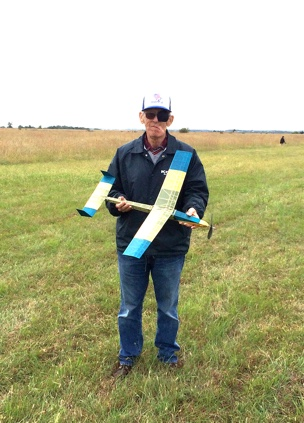
\includegraphics[width=0.45\textwidth]{../assets/images/RoieBlack.jpg}
\end{centering}

In the Summer of 1955 I was delivering the evening newspaper in Falls Church,
Virginia, when I rounded the corner of an apartment building and saw a man
release the propeller on a rubber-powered model airplane. The plane circled in
front of this man's home for several minutes, and magically landed where it had
started. The airplane was a Henderson Gadfly, published in Model Airplane News
that year.  I was fascinated by that sight, and decided to figure out how the
airplane managed to do that. I talked the man into giving me the plans he used
to build the model, traced from the magazine. I still has those plans to this
day!) Soon, a couple of my friends and I decided to start building model
airplanes of our own.  We all took a bus to downtown Washington, D.C (kids
could do that back then), and joined the Academy of Model Aeronautics. We also
joined the {\it Fairfax Model Associates} and began competing in a variety of events,
mostly control line and gas free flight. At one meeting, Bill Bigge, an
internationally known indoor model builder, was the guest speaker. I got my
first look at a new form of model airplane. The indoor models Bill brought to
the meeting were fascinating, and cheap enough even a kid with a limited
allowance could build one.  Bill became my mentor, and  I managed to build an
ornithopter and helicopter and set two national records! After almost getting a
PhD in Aerospace Engineering from Virginia Tech, I spent 20 years as an
officer in the USAF, then got a second Master's degree in Computer Science and
spent another 17 years teaching college-level Computer Science. I finally
retired for good in 2018, and moved with my wife to Kansas City, where I joined
the {\it  Heart of America Free Flight Association}, and again began flying model
airplanes, this time focusing on rubber and electric powered outdoor free
flight, and indoor events.When not building model airplanes, I am active in
Amateur Radio and am currently authoring a book on Computer Architecture.

\bibliographystyle{abbrvnat}
\tableofcontents
\bibliography{../assets/references.bib}
\end{document}
